% ******************************* Thesis Appendix A ****************************

%% **************************** Define Graphics Path **************************
%\ifpdf
%    \graphicspath{{appendixA/figs/raster/}{appendixA/figs/PDF/}{appendixA/figs/}}
%\else
%    \graphicspath{{appendixA/figs/vector/}{appendixA/figs/}}
%\fi

\graphicspath{{figs/appendixA/PDF/}}



\chapter{Examples of Uniform Time-Delay Embedding} \label{appendix:a}
Two examples regarding the methodology of uniform time-delay embedding
are presented: (A.1) using a 20 sample length vector, and
(A.2) using a time series from horizontal movement of a 
triaxial accelerometer.

\section{20 sample length vector.}
For this example, we propose to work with a vector 
$\{ \boldsymbol{x}_n \}_{n=1}^{20}$ with a sample length $N=20$ in order 
to implement an uniform time-delay embedding matrix, 
$\boldsymbol{X}^{m}_{\tau} $, with embedding dimension of $m=5$ 
and delay dimension of $\tau=3$ (Eq.~\eqref{eq:tde}).% \eqref{eq:etde_example}
The representation of the uniform time-delay embedding matrix
$\boldsymbol{X}^{5}_{3}$ is as follows
%%********************************[EQUATION]************************************
\begin{equation}\label{eq:etde_example}
\boldsymbol{X^5_3} =
\begin{pmatrix}
  \boldsymbol{ \tilde{x} }_n \\
  \boldsymbol{ \tilde{x} }_{n-3} \\
  \boldsymbol{ \tilde{x} }_{n-6} \\
  \boldsymbol{ \tilde{x} }_{n-9} \\
  \boldsymbol{ \tilde{x} }_{n-12}
\end{pmatrix}^\intercal
\end{equation}
%%********************************[EQUATION]************************************
The dimension of the uniform time-delay embedding matrix is defined by
$N-(m-1)\tau$ rows and $m$ columns.
$N-(m-1)\tau$ is also the sample length of the delayed copies of 
$\boldsymbol{x}_n$ which is equal to eight ($20-((5-1)*3)=8$).
Therefore, $\boldsymbol{X}^{5}_{3}$ can be explicitly represented as
%%********************************[EQUATION]************************************
\begin{equation}\label{eq:etdee1}
\boldsymbol{X}^5_3 =
\begin{pmatrix}
  x_1 & x_2 & x_3 & x_4 & x_5 & x_6 & x_7 & x_8 \\
  x_4 & x_5 & x_6 & x_7 & x_8 & x_9 & x_{10} & x_{11} \\
  x_{7} & x_{8} & x_{9} & x_{10} & x_{11} & x_{12} & x_{13} & x_{14} \\
  x_{10} & x_{11} & x_{12} & x_{13} & x_{14} & x_{15} & x_{16} & x_{17} \\
  x_{13} & x_{14} & x_{15} & x_{16} & x_{17} & x_{18} & x_{19} & x_{20}
\end{pmatrix}^\intercal
\end{equation}
%%********************************[EQUATION]************************************

After transposing $\boldsymbol{X}^{5}_{3}$, one can see that the ranges of
values of the uniform time-delay embedded matrix are between
$ ( (m-1)\tau )+1$  to $N$  (for this example from 13 to 20):

%********************************[EQUATION]************************************
\begin{equation}\label{eq:etdee2}
\boldsymbol{X}^5_3 =
\begin{pmatrix}
x_1 & x_4 & x_{7} & x_{10} & x_{13} \\
x_2 & x_5 & x_{8} & x_{11} & x_{14} \\
x_3 & x_6 & x_{9} & x_{12} & x_{15} \\
x_4 & x_7 & x_{10} & x_{13} & x_{16} \\
x_5 & x_8 & x_{11} & x_{14} & x_{17} \\
x_6 & x_9 & x_{12} & x_{15} & x_{18} \\
x_7 & x_{10} & x_{13} & x_{16} & x_{19} \\
x_8 & x_{11} & x_{14} & x_{17} & x_{20} \\
\end{pmatrix} =
\begin{pmatrix}
   \boldsymbol{X}[13] \\
   \boldsymbol{X}[14] \\
   \boldsymbol{X}[15] \\
   \boldsymbol{X}[16] \\
   \boldsymbol{X}[17] \\
   \boldsymbol{X}[18] \\
   \boldsymbol{X}[19] \\
   \boldsymbol{X}[20]
\end{pmatrix}.
\end{equation}
%%********************************[EQUATION]************************************

%With that in mind, the values of $\boldsymbol{X}^5_3$ in each row are the embedded
%values from $ \{  \boldsymbol{x}_n  \} $. For instance, $\boldsymbol{X}[13]$ is built
%from the following values of $ \{  \boldsymbol{x}_n  \} $:
%$ \{    x_1, x_4,x_{7},x_{10},x_{13}    \}  $.
%

%%%%%%%%%%%%%%%%%%%%%%%%%%%%%%%%%%%%%%%%%%%%%%%%%%%%%%%%
% E)eeeeee X)    xx T)tttttt R)rrrrr    A)aa
% E)        X)  xx     T)    R)    rr  A)  aa
% E)eeeee    X)xx      T)    R)  rrr  A)    aa
% E)         X)xx      T)    R) rr    A)aaaaaa
% E)        X)  xx     T)    R)   rr  A)    aa
% E)eeeeee X)    xx    T)    R)    rr A)    aa
%%%%%%%%%%%%%%%%%%%%%%%%%%%%%%%%%%%%%%%%%%%%%%%%%%%%%%%%
% It is important to note that when thinking about embedding, the down-sampled
% values of $\boldsymbol{v}_n$ are embedded into $\boldsymbol{V}[]$.
% the rows of the matrix can be viewed as down-sampled vectors by $\tau$ (three in this case).




\section{Time series for horizontal movement of a triaxial accelerometer.}
In this example, it is considered a time series of a triaxial accelerometer 
(Figure~\ref{fig:acc}(C)),
captured from repetitions of a horizontal trajectory (Figure~\ref{fig:acc}(A))
performed by user (Figure~\ref{fig:acc}(B)).
%The trajectory is indicated by the points \textbf{a} and \textbf{b} which also 
%indicate  a click sound in order to constraint the movement of the user 
%so as to be consistent and synchronised (Figure~\ref{fig:acc}(A)).
%The click sound is 60 beats per minute which means that there is a click sound
%every second, so for this experiment the beat is only reproduced for 20 seconds.
From Figure~\ref{fig:acc}(C)) is evidently that the $A_y(n)$ is 
the most affected axis of the accelerometer due to the movement's 
characteristics in the horizontal trajectory.
With that in mind, we select $A_y(n)$ as the input time series
for the uniform time-delay embedding theorem.

Considering that the sample rate of the data is 50 Hz, we propose to work
with a vector of sample length of $N=1000$ which corresponds to 20 seconds 
of data. Then, with minimum embedding parameters $m=7$ and $\tau=11$, 
the dimensions of the uniform time-delay embedding matrix, 
$\boldsymbol{{A_y}}^{7}_{11}$, are 934 ( $N-(m-1)\tau$ ) rows and 
7 ($m$) columns. 
$\boldsymbol{{A_y}}^{7}_{11}$ is therefore represented as follows:
%********************************[EQUATION]************************************
\begin{equation} \label{eq:etde1_exampleA2}
\boldsymbol{{A_y}}^{7}_{11}  =
\begin{pmatrix}
  	{ A_y }(n) \\
  	{ A_y }(n-11) \\
	{ A_y }(n-22) \\
	{ A_y }(n-33) \\
	{ A_y }(n-44) \\
	{ A_y }(n-55) \\
  	{ A_y }(n-66) 
\end{pmatrix}^\intercal
=
\begin{pmatrix}
  	a_y(1)  & \dots & a_y(934) \\
  	a_y(12) & \dots & a_y(945) \\
  	a_y(23) & \dots & a_y(956) \\
  	a_y(34) & \dots & a_y(967) \\
  	a_y(45) & \dots & a_y(978) \\
  	a_y(56) & \dots & a_y(989) \\
  	a_y(67) & \dots & a_y(1000) 
\end{pmatrix}^\intercal   
\end{equation}
%********************************[EQUATION]************************************


%********************************[EQUATION]************************************
\begin{equation} \label{eq:etde2_exampleA2}
\boldsymbol{{A_y}}^{7}_{11}  = 
\begin{pmatrix}
  	a_y(1) & a_y(12) & a_y(23) & a_y(34) & a_y(45) & a_y(56) &  a_y(67) \\ 
	\vdots & \vdots & \vdots & \vdots & \vdots & \vdots & \vdots \\
  	a_y(934) & a_y(945) & a_y(956) &  a_y(967) &  a_y(978) &  a_y(989) & a_y(1000) 
\end{pmatrix}
\end{equation}
%********************************[EQUATION]************************************

%********************************[EQUATION]************************************
\begin{equation} \label{eq:etde2_exampleA2}
\boldsymbol{{A_y}}^{7}_{11}  = 
\begin{pmatrix}
\boldsymbol{{A_y}}^{7}_{11}[67] \\
\vdots \\
\boldsymbol{{A_y}}^{7}_{11}[1000] 
\end{pmatrix}.
\end{equation}
%********************************[EQUATION]************************************






%%---------------------------------(FIGURE)-------------------------------------
\begin{figure}
 \centering
   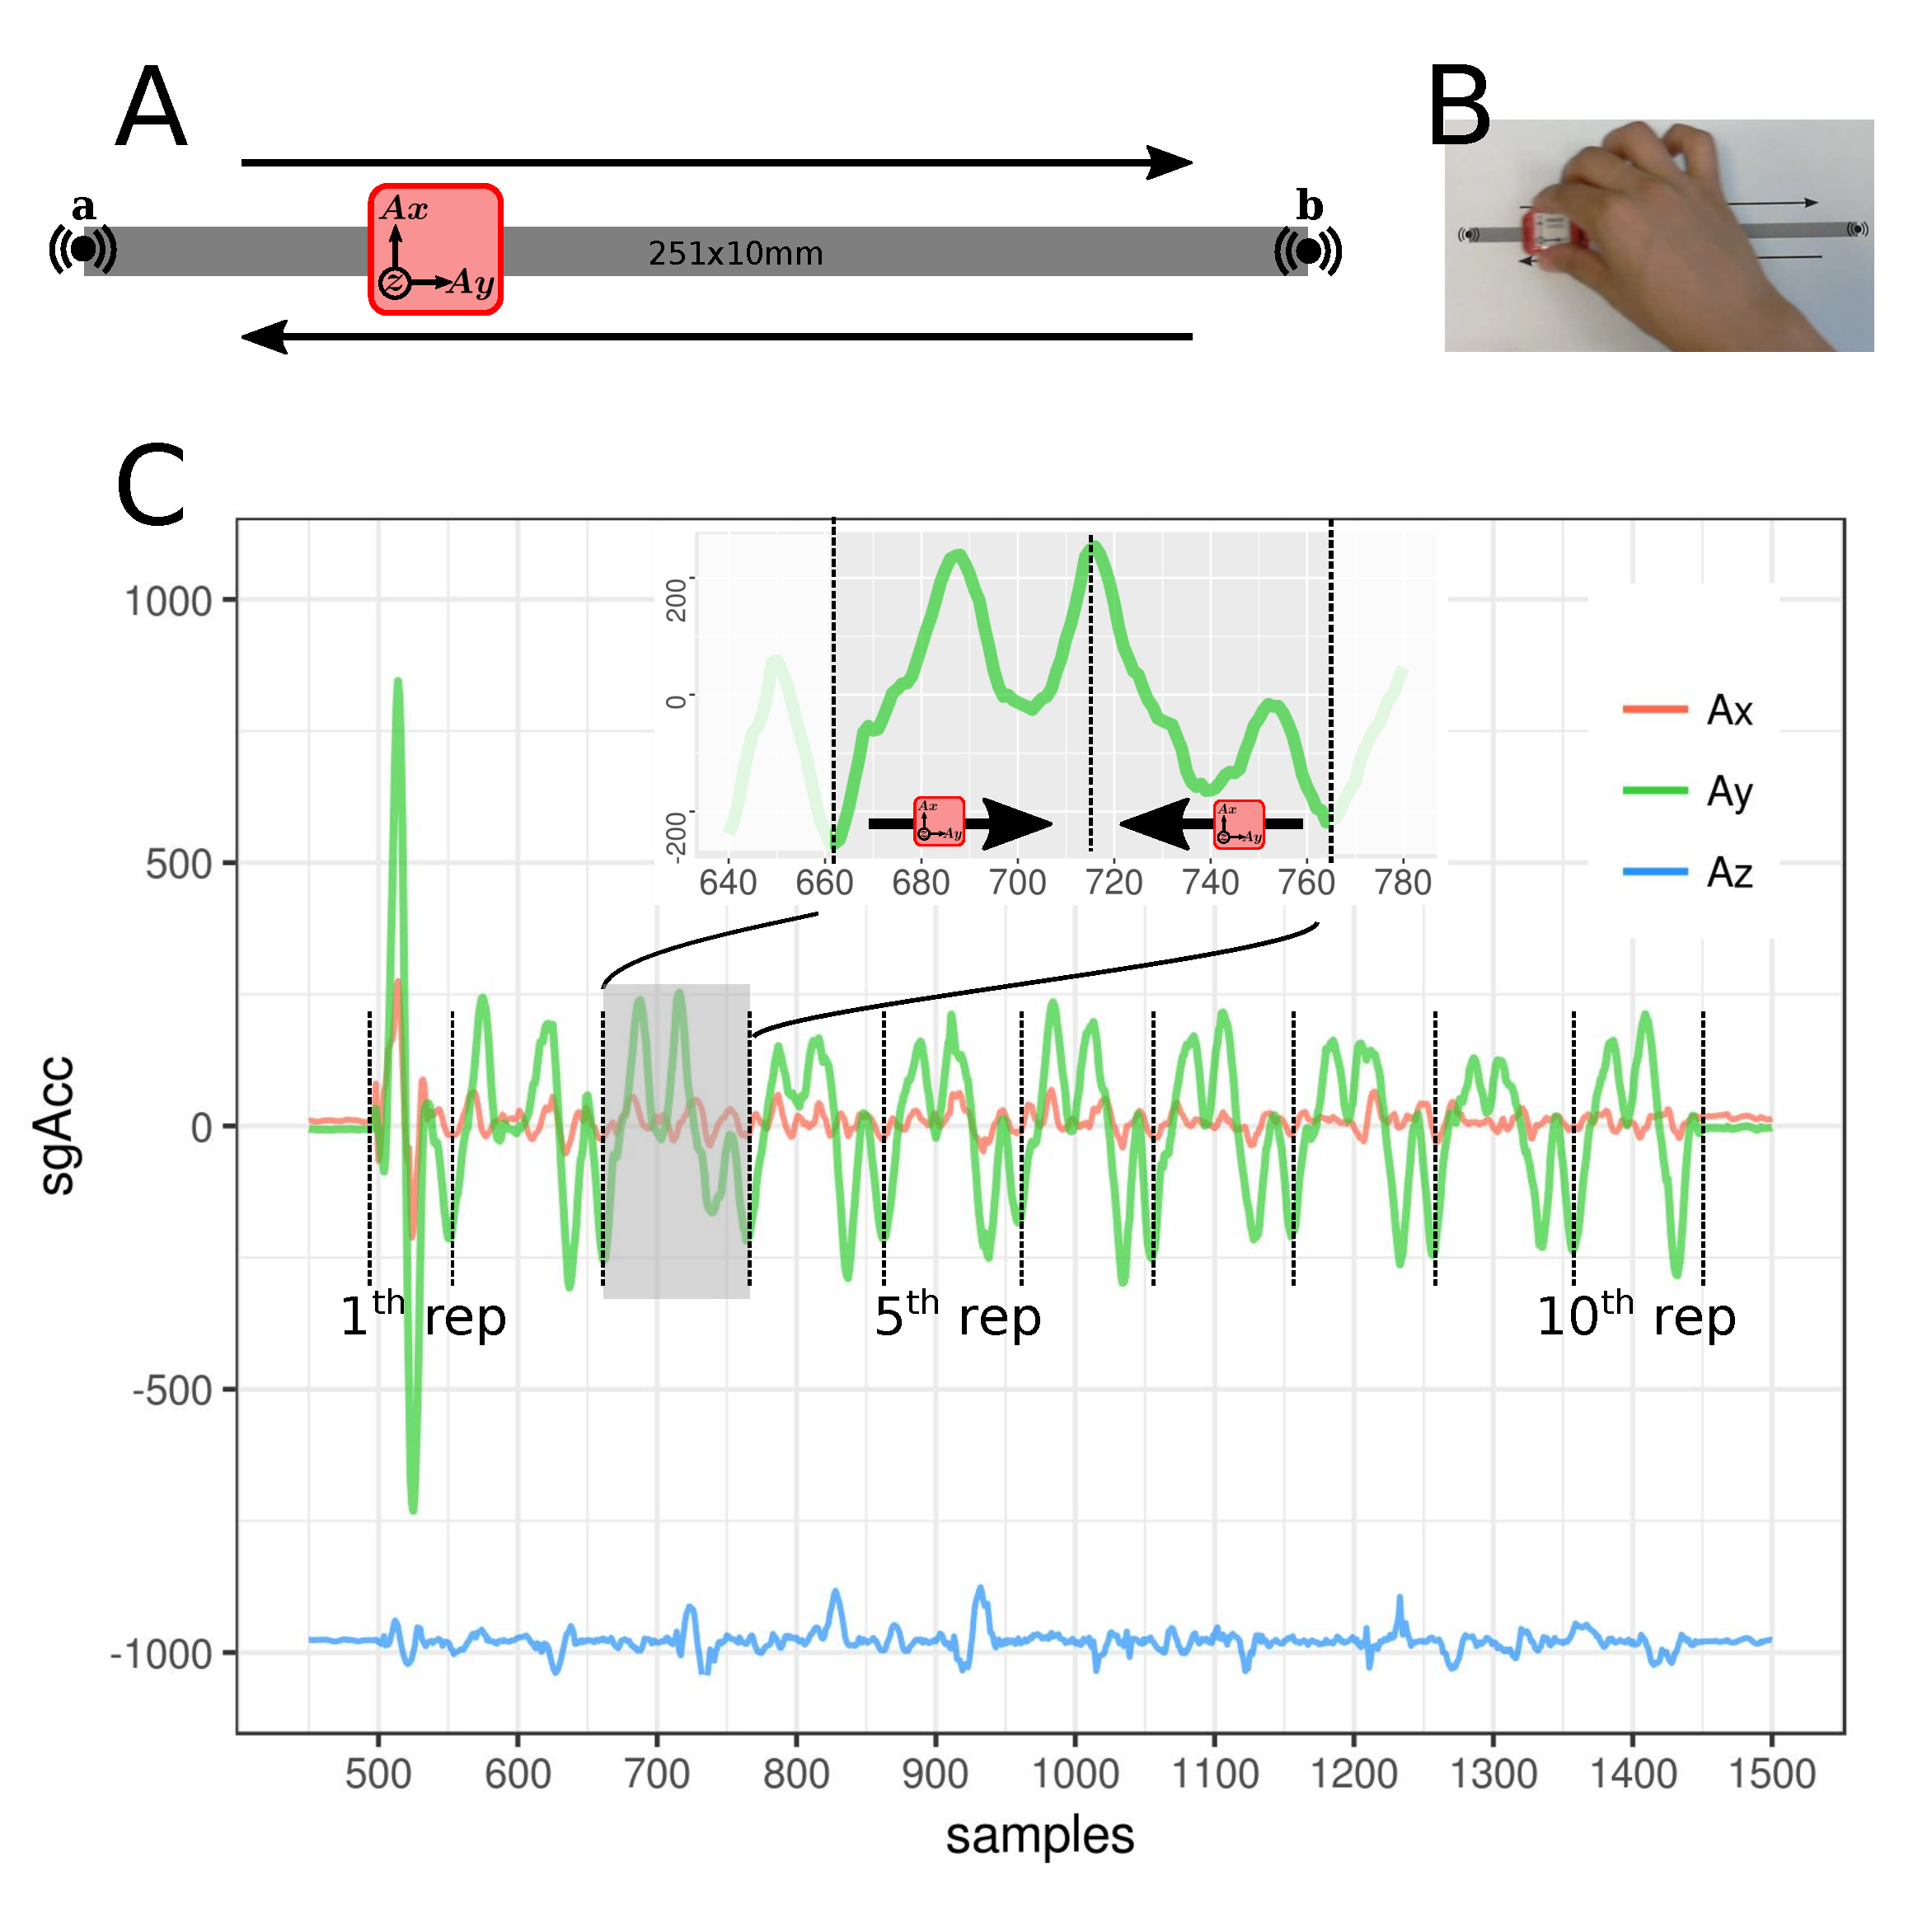
\includegraphics[width=0.8\textwidth]{hmov}
   \caption
	[Examples of time series with an IMU]{
	{\bf Example of time series with an IMU}
	(A). Triaxial accelerometer (in red) is moved repetitively across a line
   	of 251 mm from point \textbf{a} to \textbf{b} and then from
   	\textbf{b} to \textbf{a}. 
   	The points \textbf{a} and \textbf{b} indicate when a click 
	sound is produced.
	(B). Person's hand holding and moving the sensor horizontally 
	across the line.
	(C). Time series for the triaxial accelerometer 
	($A_x(n)$, $A_y(n)$, $A_z(n)$) for ten repetitive horizontal 
	movements across a line. The top time series only
   	shows $A_y$ axis which corresponds to one cycle of the 
	horizontal movement and the black arrows represent the 
	movement's direction of the accelerometer with respect 
	to the produced time series.
	}
   \label{fig:acc}
\end{figure}
%%---------------------------------(FIGURE)-------------------------------------







%
%%%---------------------------------(FIGURE)-------------------------------------
%\begin{figure}
% \centering
%   \includegraphics[width=1.0\textwidth]{figures/appendices/appendixA/sketchs_for_trajectories/figures/trajectory1a/aAhorizontal00}
%   \caption{
%	(A). Triaxial accelerometer (in red) is moved repetitively across a line
%   	of 251 mm from point \textbf{a} to \textbf{b} and then from
%   	\textbf{b} to \textbf{a}. 
%   	The points \textbf{a} and \textbf{b} indicate when a click sound is produced.
%	(B). Person's hand moving the sensor horizontally across the line.
%	}
%   \label{fig:acc}
%\end{figure}
%%%---------------------------------(FIGURE)-------------------------------------
%
%
%
%%%---------------------------------(FIGURE)-------------------------------------
%\begin{figure}
% \centering
%   \includegraphics[width=1.0\textwidth]{figures/appendices/appendixA/outcomes/figure_second_experiment/fig_2E_v03}
%   \caption{Time series for the triaxial accelerometer ($A_x(n)$, $A_y(n)$, $A_z(n)$) for
%   ten repetitive horizontal movements across a line. The top time series only
%   shows $A_y$ axis which corresponds to one cycle of the horizontal movement.
%   The black arrows with sensors represent the movement's direction of the
%   accelerometer with respect to the produced time series.
%   }
%   \label{fig:tsacc}
%\end{figure}
%%%---------------------------------(FIGURE)-------------------------------------
%
%
%





